%%
%% Commands for TeXCount
%TC:macro \cite [option:text,text]
%TC:macro \citep [option:text,text]
%TC:macro \citet [option:text,text]
%TC:envir table 0 1
%TC:envir table* 0 1
%TC:envir tabular [ignore] word
%TC:envir displaymath 0 word
%TC:envir math 0 word
%TC:envir comment 0 0
%%
%%
%% The first command in your LaTeX source must be the \documentclass command.
\documentclass[sigconf]{acmart}




\usepackage{numprint}
\npthousandsep{\,}


%% Rights management information.  This information is sent to you
%% when you complete the rights form.  These commands have SAMPLE
%% values in them; it is your responsibility as an author to replace
%% the commands and values with those provided to you when you
%% complete the rights form.
\setcopyright{acmcopyright}
\copyrightyear{2021}
\acmYear{2021}
\acmDOI{00.0000/0000000.0000000}

%% These commands are for a PROCEEDINGS abstract or paper.
\acmConference[WI-IAT '21]{Web Intelligence and Intelligent Agent Technology}{December 14--17, 2021}{Melbourne, Australia}
\acmBooktitle{WI-IAT '21: Web Intelligence and Intelligent Agent Technology December 14--17, 2021, Melbourne, Australia}
\acmPrice{15.00}
\acmISBN{000-0-0000-0000-0}

%%
%% Submission ID.
%% Use this when submitting an article to a sponsored event. You'll
%% receive a unique submission ID from the organizers
%% of the event, and this ID should be used as the parameter to this command.
%%\acmSubmissionID{123-A56-BU3}

%%
%% The majority of ACM publications use numbered citations and
%% references.  The command \citestyle{authoryear} switches to the
%% "author year" style.
%%
%% If you are preparing content for an event
%% sponsored by ACM SIGGRAPH, you must use the "author year" style of
%% citations and references.
%% Uncommenting
%% the next command will enable that style.
%%\citestyle{acmauthoryear}

%%
%% end of the preamble, start of the body of the document source.
\begin{document}

%%
%% The "title" command has an optional parameter,
%% allowing the author to define a "short title" to be used in page headers.
\title[Embedding Multiple Facets of Long Texts]{Novel Views on Novels:\\Embedding Multiple Facets of Long Texts}

%%
%% The "author" command and its associated commands are used to define
%% the authors and their affiliations.
%% Of note is the shared affiliation of the first two authors, and the
%% "authornote" and "authornotemark" commands
%% used to denote shared contribution to the research.
\author{Lasse Kohlmeyer}
\email{lasse.kohlmeyer@student.hpi.de}
\affiliation{%
  \institution{Hasso Plattner Institute}
  \country{University of Potsdam, Germany}}

\author{Tim Repke}
\orcid{0000-0001-9661-6325}
\email{tim.repke@hpi.de}
\affiliation{%
	\institution{Hasso Plattner Institute}
	\country{University of Potsdam, Germany}}

\author{Ralf Krestel}
\orcid{0000-0002-5036-8589}
\email{ralf.krestel@acm.org}
\affiliation{%
  \institution{ZBW Leibnitz Information Centre for Economics}
  \country{Kiel University, Germany}}


%%
%% By default, the full list of authors will be used in the page
%% headers. Often, this list is too long, and will overlap
%% other information printed in the page headers. This command allows
%% the author to define a more concise list
%% of authors' names for this purpose.
\renewcommand{\shortauthors}{Kohlmeyer, et al.}

%%
%% The abstract is a short summary of the work to be presented in the
%% article.
\begin{abstract}
Novels are one of the longest document types and thus one of the most complex types of texts.
Many NLP tasks utilize document embeddings as machine-understandable semantic representations of documents.
However, such document embeddings are optimized for short texts, such as sentences or paragraphs.
When faced with longer texts, these models either truncate the long text or split it sequencially into smaller chunks.
We show that when applied to a fictional novel, these traditional document embeddings fail to capture all its facets.
Complex information, such as time, place, atmosphere, style, plot, and content are typically not represented adequately.

To this end, we propose \emph{lib2vec} which computes and combines multiple embedding vectors based on various facets.
Instead of splitting the text sequencially, \emph{lib2vec} splits the text semantically based on domain-specific facets.
We evaluate the semantic expressiveness using human-assessed book comparisons as well as content-based information retrieval tasks.
The results show that our approach outperforms state-of-the-art document embeddings for long texts.
\end{abstract}

%%
%% The code below is generated by the tool at http://dl.acm.org/ccs.cfm.
%% Please copy and paste the code instead of the example below.
%%
%\begin{CCSXML}
%<ccs2012>
% <concept>
%  <concept_id>10010520.10010553.10010562</concept_id>
%  <concept_desc>Computer systems organization~Embedded systems</concept_desc>
%  <concept_significance>500</concept_significance>
% </concept>
% <concept>
%  <concept_id>10010520.10010575.10010755</concept_id>
%  <concept_desc>Computer systems organization~Redundancy</concept_desc>
%  <concept_significance>300</concept_significance>
% </concept>
% <concept>
%  <concept_id>10010520.10010553.10010554</concept_id>
%  <concept_desc>Computer systems organization~Robotics</concept_desc>
%  <concept_significance>100</concept_significance>
% </concept>
% <concept>
%  <concept_id>10003033.10003083.10003095</concept_id>
%  <concept_desc>Networks~Network reliability</concept_desc>
%  <concept_significance>100</concept_significance>
% </concept>
%</ccs2012>
%\end{CCSXML}
%
%\ccsdesc[500]{Computer systems organization~Embedded systems}
%\ccsdesc[300]{Computer systems organization~Redundancy}
%\ccsdesc{Computer systems organization~Robotics}
%\ccsdesc[100]{Networks~Network reliability}

%%
%% Keywords. The author(s) should pick words that accurately describe
%% the work being presented. Separate the keywords with commas.
%\keywords{datasets, neural networks, gaze detection, text tagging}

%%
%% This command processes the author and affiliation and title
%% information and builds the first part of the formatted document.
\maketitle

\section{Introduction}
Reading is one of the main strategies to obtain new information.
However, the availability and the amount of information are continuously growing.
This is not only the case for news articles or user-generated content such as online comments but also for books~\citep{wu_mind_2020, roser_books_2013, fink-jensen_book_2015}.
For example, in 2019, \numprint{78746} new books were published in Germany~\citep{lippmann_buchproduktion_2019} and \numprint{1600000} books were self-published in the USA in 2018~\citep{bowker_self-publishing_2019}.
These numbers clearly illustrate the so-called \textit{information overload problem}~\citep{wang_literature_2020, alharthi_survey_2018} which applies to book publishers and readers alike.
Automatic methods can assist human decision making, for example book publishers who have to select books from a large number of submitted manuscripts by judging whether they align with their program and potential commercial success~\cite{ashok_2013}.

Machine-understandable representations of books are the basis for such automated approaches.
Numerical representations can be used to calculate similarities between books as well as for clustering, classification or content-based recommender systems.
Modern document embeddings are usually designed to encode shorter texts.
For example BERT~\citep{devlin_bert_2019} is limited to \numprint{512} tokens, Longformer~\citep{beltagy_longformer_2020}, which is designed for long sequences, is limited to \numprint{4096} tokens, and doc2vec has a limit of \numprint{10000} while books may easily exceed \numprint{100000} tokens.
Furthermore, there are hardly any publications that process the full-text of books holistically~\citep{alharthi_study_2019}.
However, full-text is one of the key characteristics of a book and should be considered when encoding a book.

To this end, we propose \emph{lib2vec}\footnote{Based on the Latin word for book: liber.} which embeds subsets of words of a book individually using state-of-the-art embedding algorithms.
These subsets, which we associate with \emph{facets}, represent different angles, views, or aspects of a book.
In the context of novels, which is the focus of this study, possible facets of interests are the plot, where and when the plot is set, the novel's atmosphere, its content, and style.
To compute these facet embeddings, we identify words in the text corresponding to facets and construct pseudo-documents.
Each facet embedding can be used individually for applications that need to compare aspects of a novel.
We also examine strategies to combine facet embeddings into a single embedding vector for a novel.

We evaluate the performance of our approach on different tasks with multiple English and German corpora of novels and compare it to a number of state-of-the-art embedding models.
Our experiments show that \emph{lib2vec} is able to significantly outperform other models in determining author and genre similarity as well as identifying books belonging to the same series, such as Harry Potter sequels.
In addition, we evaluate our embedding on genre and rating prediction of novels.
Furthermore, we introduce the \emph{BoCo} dataset with similarities between 20 books under different aspects annotated by \numprint{81} domain experts.

Our contribution can be summarized as follows:
(1) We present \emph{lib2vec}, a framework which computes and combines multiple embedding vectors based on various facets. Instead of splitting the text sequencially, \emph{lib2vec} splits the text semantically based on domain-specific facets.
(2) \emph{lib2vec} provides memory and time-efficient computation of embedding vectors for long texts.
(3) \emph{lib2vec} allows the comparison of books with respect to different facets.
(4) We compare \emph{lib2vec} to competitive baselines in a wide range of experiments.
(5) We introduce a new benchmark dataset to evaluate book similarities.

\section{Related Work}

%A language model is central for various Natural Language Processing (NLP) applications.
%Some example scenarios are speech recognition~\citep{povey_kaldi_2011, arisoy2012deep}, machine translation\citep{schwenk2012large, vaswani2013decoding, conneau2019cross}, text summarization\citep{rush2015neural, filippova2015sentence, liu_text_2019}, or text generation~\citep{lebret2016neural,fedus2018maskgan,  dong_unified_2019}.
%Language models learn a probability distribution over sequences of words or characters.
%This means a language model can assign each sequence of words a probability score which could be used to predict the next likely word of a sequence~\citep{jozefowicz_exploring_2016}. 
%Before a language model can be created by a computer it is necessary to convert human language into a machine-readable representation.
Semantically meaningful book representations are closely related to word and document embeddings.
Word embeddings, such as word2vec~\citep{mikolov_efficient_2013}, quickly gained popularity, as they provide a dense vector representation for words that can be used to, e.g., calculate the semantic similarity between words.
\citet{grayson_novel2vec_2016} apply word2vec on 19th-century novels to investigate to which extend quantitative literary analysis can profit from the semantic similarities between word embeddings in their approach \emph{novel2vec}.
A big difference to our \emph{lib2vec} framework is that no novel representation is obtained by \emph{novel2vec}.
However, such an encoding of a book is calculated by ~\citet{anvari_book2vec_2018}.
Their approach \emph{book2vec} uses the reading histories of users to model sequences of books which serve as input for the word2vec algorithm. 
In contrast to \emph{book2vec}, \emph{lib2vec} is applied on the texts of novels, which is not dependent on user-data such as reading histories.
%More recently, context-sensitive embedding approaches, such as BERT~\citep{devlin_bert_2019},	% RoBERTa~\citep{liu2019roberta}, XLM~\citep{conneau2019cross}, or Flair~\citep{akbik_contextual_2018},
%were introduced.
%As opposed to traditional word embeddings, these methods do not produce a static vector for each word, but compute a representation for each word depending on its context.

To utilize word embeddings in full-text applications, \citep{le_distributed_2014} introduced paragraph embeddings for short texts.
However, their input sequence is limited and longer texts need to be trunkated, which leads to a loss of information and poor performance for long, heterogeneous texts.
Modern, transformer-based document embedding algorithms have a much higher limit by utilizing an internal self-attention mechanism to capture contextual information of entire documents~\cite{DBLP:journals/corr/abs-1904-10509, DBLP:conf/emnlp/QiuMLYW020, DBLP:conf/iclr/KitaevKL20}.
However, these models are typically task specific and the attention mechanism has very high computation and memory requirements.
For example, the most recent Longformer model requires multiple powerful GPUs with 48GB RAM to cover documents of up to 32K tokens~\citep{beltagy_longformer_2020}.
%
%In practice, modern document embedding algorithms have an input sequence limit since embedding sequences that are too long are inefficient in terms of computation time and memory requirements~\citep{beltagy_longformer_2020}.
%Thus, document embeddings truncate texts to their input sequence limits which leads to a loss of information and poor performance for long, heterogeneous texts.


{P-SIF} was introduced to embed longer documents~\citep{gupta_p-sif_2020}.
It considers the topical structure of documents by concatenating word embeddings over the topic distribution of words. 
%These word topic vectors are weighted by TF-IDF to cluster them into different partitions. 
{P-SIF} has similarities to our work, since in both algorithms embeddings for a fixed number of selected groups of words are computed. 
However, in contrast to our work, only topical information of a text is utilized by {P-SIF} and not other kinds of information such as style or location.
Furthermore, {P-SIF} is evaluated on news articles or reviews that are much shorter than novels.

Other downsides of existing document embedding approaches are the poor performance in classification tasks and the lack of interpretability of the latent vector space.
Both are adressed by \citet{unnam_document_2020}, who utilize words with high discriminatory power as dimension features for the latent space of documents which improves classification performance and interpretability.
We show that by embedding multiple facets our approach addresses these issues as well. %multiple vectors offer more possibilities for information encoding and more fine-grained semantic representations. 
%Alternative approaches of document embeddings include Word Mover's Embeddings~\citep{wu_word_2018}. 
%The authors utilize the \textit{Word Mover's Distance} by~\citet{kusner2015word} which measures the distance of documents by the distance of word embeddings in that documents.
%The document embedding is calculated by the smallest distance that the embedded words of one document must ``travel'' to reach the embedded words of another document~\citep{wu_word_2018}.

Multi-view learning or multi-faceted embeddings refer to the same family of approaches and are often motivated by the polysemy of words~\citep{neelakantan_efficient_2014}.
Multi-faceted text embeddings often use different data sources.
These different data sources are, e.g., utilized to achieve a higher quality for general word embeddings~\citep{luo_pre-trained_2014} or domain-specific word embeddings~\citep{rettig_fusing_2019}.
Thereby, embeddings of the same word based on different data sources serve as independent facets.
The facets are combined by dimensionality reduction based on neural networks~\citep{luo_pre-trained_2014} or PCA~\citep{rettig_fusing_2019}.
Nevertheless, a minority of works create facets from the same data source.
In this area,~\citet{neelakantan_efficient_2014} train embeddings that capture the polysemy of words.
Starting with the word to be embedded, the authors cluster the surrounding context words into word sense clusters.
Afterward, they embed each of the sense clusters separately to form the different facets.
Very similarly, \emph{lib2vec} uses the same text data to form different facets.
However, instead of word embeddings, \emph{lib2vec} calculates document embeddings, and instead of word context clustering to obtain sets of words, it selects words by leveraging annotations such as part-of-speech tags.

To create different facets of documents, other information such as click or interaction data can be used in addition to text data~\citep{sang_multi-modal_2019,li_multi-view_2019}.
Thus, most text-related multi-faceted embeddings leverage facets based on auxiliary data apart from \citet{risch_book_2018}.
To encode book synopses, they embed three different facets: time, place, and plot.
While for the time embedding they trained a classifier that assigns a year to each synopsis, for the location they average the word embeddings of all location words. 
Only the representation of the plot is obtained by doc2vec.
In contrast, \emph{lib2vec} computes all facet embeddings in a unified way, using one and the same document embedding algorithm, e.g., doc2vec.
Instead of having to train an additional classifier or use other external information, the information contained in the text is leveraged. 
Thus, new facets can be constructed with less effort.
Another difference to \citet{risch_book_2018} is the selected data, as synopses are much shorter than novels and provide other possibilities for facets.

Besides multi-faceted embeddings, there are other ways to encode novels.
Many of these approaches are based on hand-crafted features such as readability~\citep{pera_what_2013}, stylometric features for authorship attribution~\citep{alharthi_authorship_2018}, as well as token/type ratios, word frequencies, or the number of female characters within a text~\citep{alharthi_study_2019}.
A disadvantage of hand-crafted features is that they are often very domain-specific and are difficult to transfer to other scenarios.
In contrast to hand-crafted features, \emph{lib2vec} generates different facets in an unsupervised manner, based on annotations. 
While they are also not domain-independent, they can be customized with less effort, as only relevant annotations need to be identified.

\citet{maharjan_multi-task_2017} show that hand-crafted features such as character n-grams are often outperformed by neural-network-based approaches.
The authors obtain full-text representations of books based on various strategies, e.g., feature-based or based on document embeddings. % such as word-level features, such as bigrams and neural embeddings by pre-trained word embeddings, doc2vec, and an RNN.
They created a Goodreads~\footnote{\url{https://www.goodreads.com/}} dataset which contains annotations for success, in form of ratings, and genre. 
We use this dataset for testing rating and genre classification.
To tackle the input sequence limit of document embedding algorithms, the authors represented each sentence as the average of its word embeddings and then fed chunks of 128 of these vectors into a multi-layer RNN to get a representation for the whole text as a result.
In contrast, \emph{lib2vec} does not apply chunking, since it leads to a loss of information and therefore to poor quality of embeddings. %citation needed! or we need to include some numbers in the evaluation (maybe for CRV)
The experiment by~\citet{maharjan_multi-task_2017} is adopted by~\citet{khalifa_will_2020}, who created book encodings by sentence embeddings incorporating readability scores.
Again, our approach differs, because our strategy for dealing with long documents is less affected by the loss of information when different sentence embeddings are aggregated.

%While~\citet{benton_learning_2016} obtain optimal weights for each facet by Canonical Correlation Analysis (CCA) for downstream tasks in the area of user classification and friend recommendation,~\citet{sang_multi-modal_2019} utilize a topic model to merge question pairs with network data, and~\citet{li_multi-view_2019} merge the results from different obtained facets to identify relevant emails.
%Experiments showed that word embeddings can capture semantic relationships of book characters~\citep{grayson_novel2vec_2016} for a small corpus containing twelve books by three 19th century authors.

\section{Multi-Faceted Document Embeddings}

\begin{figure}
	\centering
	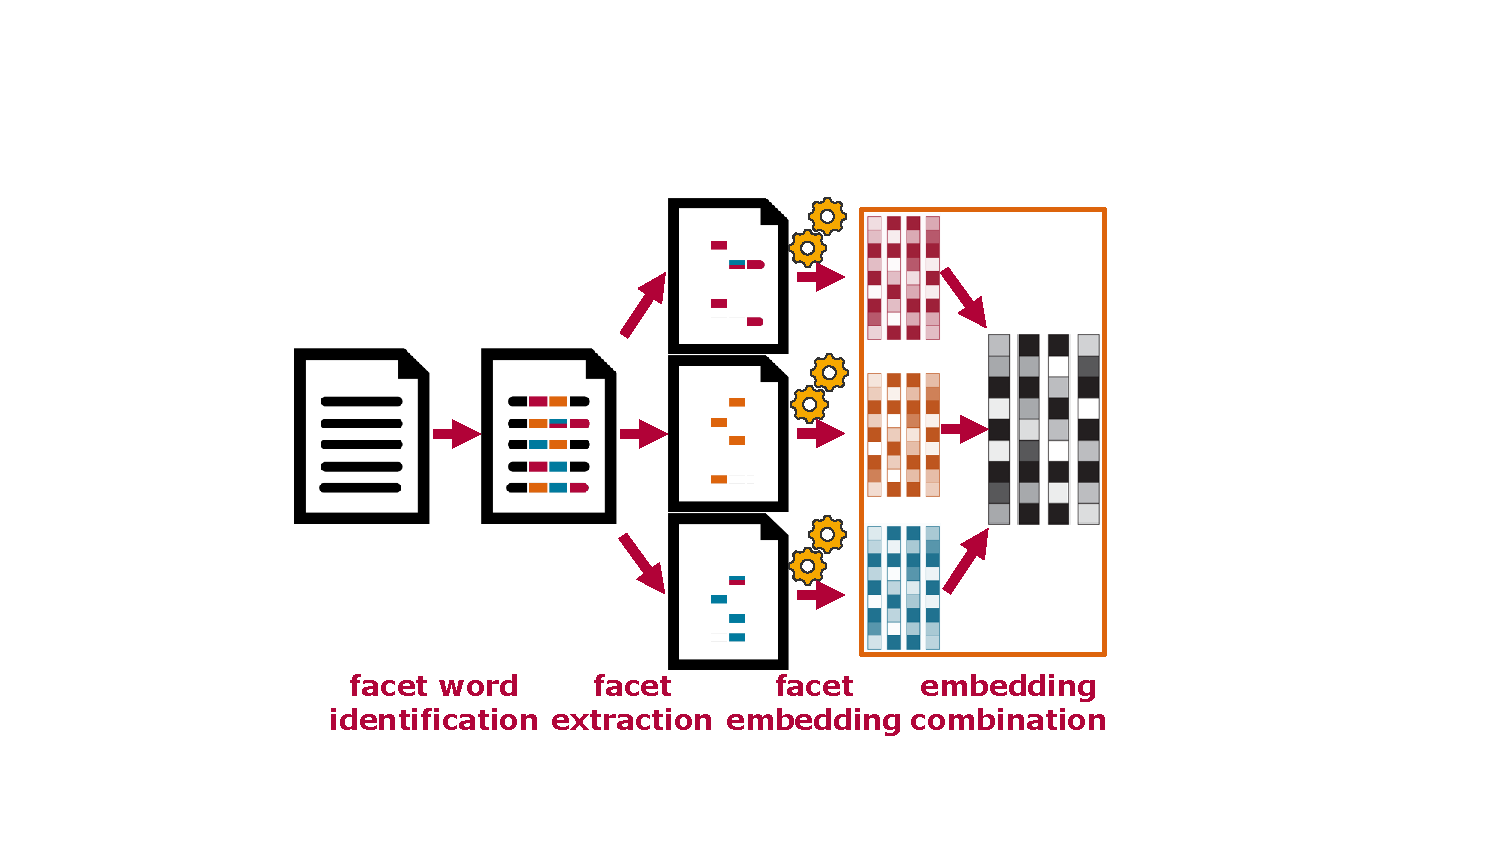
\includegraphics[width=0.99\linewidth]{figures/approach_overview.pdf}
	\caption{Overview of the four main processing steps of \emph{lib2vec}.}
	\label{fig:overview}
\end{figure}

Embeddings for long documents are typically realized by splitting them into smaller parts following either a truncation-based, chunk-based, or a facet-based strategy.
Truncation-based approaches are using only the first $n$ words of a text, where $n$ corresponds to the input sequence limit of the embedding algorithm.
%As a downside, most of the words in a book are not used to obtain a representation, which can result in a poor embedding quality.
Chunk-based approaches split a text into several segments of size $n$ with $n\leq$ input sequence limit.
Then, each segment is embedded separately and then combined, for example via summation.
%Despite the complete full-text can be considered with the chunk-based strategy, a downside could be an increased calculation time because more data need to be processed.
%Furthermore, all books could consist of different numbers of chunks, which leads to less flexibility and more information loss during the combination of chunks.
%A consequence of this information loss is a poor quality of the obtained embedding.
Both these strategies loose crucial information either by ignoring large parts of the text (truncation) or by averaging intermediate results (chunking).
To overcome thes disadvantages, we propose \emph{lib2vec} which follows the idea by \citet{risch_book_2018} and divides a text into several facets, instead of chunks.
The novel core idea of \emph{lib2vec} is to split long texts not sequencially based on document position but rather selectively based on semantic facets

We define facets as subsets of words following semantic categories.
In this work, these categories are oriented toward the perspectives of literary analysis such as atmosphere or style.
Thereby, each category includes certain words, for example, the style facet includes stopwords since there usage is a good indicator for different styles.
Besides, words that appear in one facet may also appear in another facet.
Compared with truncation-based approaches, facet-based approaches make use of more words of a text.
While the number of chunks differs for each text, the number of facets is constant for any text.
In addition, facets are semantically meaningful, while chunks only provide information about the position within a text.

\subsection{Processing Pipeline of lib2vec}

Figure~\ref{fig:overview} illustrates the overall concept for our multi-faceted embedding approach: identifying candidate words, constructing pseudo-documents, and computing embeddings.

\paragraph{Facet Word Identification.}
In the first step, documents are preprocessed with sentence splitting, tokenization, lemmatization, POS-tagging, named entity recognition (NER), and semantic word dictionary lookups.
Each book in a corpus is annotated automatically, using SpaCy~\citep{honnibal2020spacy}, Heideltime~\citep{stroetgenmultilingual2013}, the German semantic dictionary GermaNet~\citep{hamp1997germanet, henrich2010gernedit}, and the English semantic dictionary WordNet~\citep{fellbaum2010wordnet}.
%While SpaCy extracts sentences, tokenizes texts, lemmatizes words, and assigns POS- and NER-tags, Heideltime is specialized for temporal named entities.
%GermaNet and WordNet identify abstract place, time, and atmosphere descriptors for the \emph{lib2vec} extensions \textit{Net} and \textit{Net Only}.
%While the Net extension combines these descriptors with POS-tags and named entities, the Net Only variant exclusively utilizes the semantic dictionaries.

\paragraph{Facet Extraction.}
In this step, words in a document are assigned to none, one, or multiple of the facets \textit{time}, \textit{place}, \textit{style}, \textit{atmosphere}, \textit{plot} or \textit{content}.
Additional facets can be defined in the future if necessary.
%Previous annotations are used to identify and assign facet words.
%In some cases, the actual context of a selected word may be lost. 
%This loss of context can cause problems in context-sensitive embedding algorithms.
%To preserve the context, an additional word window of length $w$ can be added around the actual facet word to the set of the facet words.
%Preserving the context by this mechanism is referred to as \textit{window extension}.
For each facet, a pseudo-document is generated containing all assigned words.
%In order to find the correct numeric encoding for a specific facet of a document, a unique identifier is created for each pseudo-document.
%The identifier contains the original document identifier as well as an identifier for the represented facet.
%Thus, the created identifier enables the individual targeting of document facets for all books.

\paragraph{Facet Embedding.}
Each pseudo-document consists of only a fraction of the words of the original book.
This allows to compute facet-specific embeddings using existing document embedding approaches.
%To encode a facet, which means, to encode the pseudo-document constructed of the associated facet-words, the pseudo-document is passed to an embedding algorithm.
%In other words, the embedding algorithm processes all facet-based pseudo-documents instead of the original full-texts.
%Compared with truncation-based algorithms, \emph{lib2vec} can use more words of the full-text.
%The number of documents, as well as the number of words that the algorithm has to process, is thus increased.
%Since the algorithm has more data available, this increase can already improve the quality of the results.
%Theoretically, any document embedding algorithm can be used in this step.
We opted for using doc2vec since it has the largest input sequence limit.
In case the pseudo-document exceeds this limit, the facet is truncated.
%Alternatively, instead of truncation, the facet can be chunked.

\subsection{Facet Definitions}
As described earlier, we use the tagged documents to construct pseudo-documents for each facet.
In this section, we describe in more detail how these pseudo-documents are compiled.

\paragraph{Location.}
The location facet is based on tokens that are tagged as geopolitical locations and buildings by SpaCy NER.
%This is a major difference to \citet{risch_book_2018}, who obtained an averaged vector of pre-trained embeddings of location words.
Multiple appearances of a word are kept to preserve their frequency, as intermittently reappearing places may be more important to the book.
%The same applies to other facets as well.
A downside of NER is, that unnamed places such as \textit{ocean}, \textit{garden}, or \textit{street} are not included.
Thus, we use GermaNet or WordNet to identify location descriptors.
%GermaNet and WordNet contain specific groups of words, for example, \textit{location} or \textit{emotion}.
%Each lemmatized word form in these groups is added to the pseudo-document if it occurs in the current book text for the \textit{Net} and \textit{Net Only} variants.

\paragraph{Time.}
Similar to location, we use NER to construct the pseudo-document for the time facet.
Although this covers months, seasons, or year numbers, phrases referring to historical events such as revolutions or wars are not tagged by standard NER tools.
Thus, we again utilise  GermaNet or WordNet to extend the scope to include events and abstract time descriptors.

\paragraph{Style.}
Prior studies have shown correlations between authorship attribution, the style of a text, and the usage of stopwords~\citep{arun_stopword_2009, tausczik_psychological_2010, alharthi_authorship_2018}. 
Following these findings, we construct the style facet based on all stopwords found by a POS-tagger.
Since stopwords appear very frequently, we expect this pseudo-document to grow quickly.
Although this might be problematic considering sequence length limitations of embeddings, we assume that truncated stopwords are already present in the limited sequence and the potential loss of information is small.

\paragraph{Atmosphere.}
Adjectives and adverbs are common linguistic indicators of the atmosphere of a text, since they describe the properties of objects, people, or emotions.
In addition, affective or sensual words such as \textit{gloomy}, \textit{warm}, \textit{smell}, or \textit{howl} also have a great influence on the atmosphere~\citep{tausczik_psychological_2010}.
In order to take these affective and sensual words into account, we consider nouns, verbs, and adjectives corresponding to emotions and feelings as identified by GermaNet or WordNet.

\paragraph{Plot.}
We utilise the basic assumption that the plot of a novel describes the actions between characters~\citep{labatut_extraction_2019, lee_story_2020}.
Such actions are expressed by verbs and adverbs.
Thus, we construct the pseudo document for the plot facet based on words with these POS-tags.

\paragraph{Content.}
We use topic modelling to construct the pseudo-document for the content facet.
Topic modelling has been shown to be useful for analyzing literary texts~\citep{uglanova_2020}.
Due to its high computational costs, we only include this facet for the book comparison task (Section~\ref{ssec:bookComparisons}.
We trained an LDA~\citep{blei2003latent} topic model on the input corpus and set the number of topics to 15.
Afterwards, we use the top 100 associated words of the five most relevant topics of a book according to the inferred topic distribution.
Given that topic modelling plays only a minor part in \emph{lib2vec} we treat it as a black box and defer further analysis to future work.

\paragraph{Raw.}
In addition, we also include a full-text facet containing the beginning of a book without any filtering apart from the truncation after the maximum sequence length.
In contrast to other facets, the raw facet preserves continuous text and word order which may improve the results if the applied document embedding algorithm can take advantage of such textual continuities.


\subsection{Combination of Facets}

In the previous sections we described the construction of pseudo-documents for facets.
For practical reasons and in order to compare our approach to other document embedding methods, we need to combine the facet embeddings into a single vector.
\citet{rettig_fusing_2019} cover a number of approaches of aggregating embedding vectors for their multi-faceted word embeddings.
The na\"ive approach to combine facet embeddings is to use the arithmetic mean (AVG) or an element-wise sum of the individual vectors.
\citet{gittens_skip-gram_2017} have empirically shown that the summation of word and document embeddings can retain aspects of two underlying embedding vectors.
Another approach is to simply concatenate facet embedding vectors (CONCAT).
This has the advantage that facet embeddings can have a different dimensionality and the information captured by each facet is still available in the resulting vector.

We propose to combine concatenation with dimensianality reduction to benefit from more encoded information while keeping the dimensionality low.
To this end, we used principal component analysis on the concatenated vectors (PCA).
We also experimented with other dimensionality reduction methods, such as autoencoders, but results were worse compared to the PCA.
And PCA has the advantage, that it can be computed very efficiently.
However, projecting previously unseen books into the low-dimensional space is not easily possible.
Another downside of dimensionality reduction in general is that a rather large corpus is necessary to identify the latent dimensions. 
Furthermore, the resulting embeddings cannot be used for semantic operations using facet encodings.
In the experiments, we report results for three different combination methods: AVG, CONCAT, and PCA.

\section{Experimental Setup}

In this section we provide an overview of which datasets we use for our evaluation, how we mitigate the influence of potential biases in our experiments, and describe the baselines we compare our approach to.

\subsection{Datasets}

%\renewcommand{\tabcolsep}{3.7pt}
%\begin{table}
%	\centering
%	\footnotesize
%	\begin{tabular}{L{0.87cm}L{0.64cm}R{0.63cm}R{0.76cm}R{0.77cm}R{0.71cm}R{0.7cm}R{0.65cm}}
%		\toprule
%		Dataset & Language & \# Books & \# Words & \# Unique Words & $\varnothing \#$ Words per Book  & $\varnothing \#$ Unique Words per Book & $\varnothing \#$ Books per Author \\
%		\midrule
%		CGF    & GER      & 3.2K    & 204M            & 26M       & 46K          & 7.2K                    & 5.7                \\
%	%	S-CGF  & GER      & 208      & 22.2M          & 2.63M      & 81.4K         & 11.1K                    & 4.24                \\
%		DTA    & GER      & 459      & 26M           & 4M        & 44K         & 7.5K                    & 2.1                \\
%%		LitRec & EN       & 3.1K    & 275M            & 22M       & 73K          & 7.0K                    & 2.8                \\
%		MGG    & EN       & 1K       & 17M           & 3M        & 17K         & 2.8K                    & 2.1                \\
%		BoCo    & EN       & 20       & 4M             & 198K    & 145K             & 8.9K                    & 1.2       \\
%		\bottomrule
%	\end{tabular}
%	\caption[Overview of Different Dataset Characteristics]{Overview of dataset characteristics.
%		The number of books for each corpus and its language, values for word counts and vocabulary sizes are reported. The median is reported for the amount of words per book and the mean for the amount of books per author.}
%	\label{tab:datasets_overview}
%\end{table}

\begin{table}
	\centering
	\caption[Overview of Dataset Characteristics]{Overview of dataset characteristics}
	\label{tab:datasets_overview}
	\begin{tabular}{crrrr}
		\toprule
		Dataset                                			& CGF  & DTA  & MGG  & BoCo  \\
		\midrule
		$\text{Language}$                               	& GER  & GER  & EN   & EN   \\[0.2em]
		$\text{\# Books}$                               	& 3.2K & 459  & 1K   & 20   \\[0.2em]
		$\text{\# Words}$                               	& 204M & 26M  & 17M  & 4M   \\[0.2em]
		$\text{\# Unique Words}$                        	& 26M  & 4M   & 3M   & 198K \\[0.2em]
		$\frac{\text{\# Words}}{\text{per Book}}$	 	& 46K  & 44K  & 17K  & 145K \\[0.2em]
		$\frac{\text{\# Unqiue Words}}{\text{per Book}}$	& 7.2K & 7.5K & 2.8K & 8.9K \\[0.2em]
		$\frac{\text{\# Books}}{\text{per Author}}$     	& 5.7  & 2.1  & 2.1  & 1.2  \\
		$\frac{\text{\# Books}}{\text{per Series}}$     	& 2.5  & 3.2  & --  & --  \\
		\bottomrule
	\end{tabular}
\end{table}

\begin{table}
	\centering
	\caption[Overview of Facet Coverage]{Overview of average facet coverage values}
	\label{tab:facet_stats}
\begin{tabular}{crrrr}
	\toprule
	Facet &    CGF &    DTA &    MGG &   BoCo \\
	\midrule
	Atmosphere &  0.144 &  0.142 &  0.106 &  0.110 \\
	Location   &  0.012 &  0.015 &  0.006 &  0.004 \\
	Plot       &  0.183 &  0.179 &  0.167 &  0.184 \\
	Raw        &  1.000 &  1.000 &  1.000 &  1.000 \\
	Style      &  0.479 &  0.465 &  0.470 &  0.505 \\
	Time       &  0.007 &  0.006 &  0.010 &  0.009 \\
	\bottomrule
\end{tabular}
\end{table}

Key characteristics of the datasets used are provided in Table~\ref{tab:datasets_overview}.
The median is reported for the average number of (unique) words per book and the mean for the average number of books per author.
An overview of the average coverage for each facet is provided in Table~\ref{tab:facet_stats}.
The average coverage is calculated by averaging the ratio of facet tokens and the number of total tokens per document over the corresponding corpus. 

\paragraph{Corpus of German-Language Fiction (CGF).}
The Corpus of German Fiction by~\citet{fischer_corpus_2017} consists of \numprint{3219} German prose books published between 1840 and 1930.
%The vast majority of books (\numprint{2735}) were written by 549 German authors, the others are translated into German as they were originally published in by 18 English, Russian, and French authors.
For our series classification task, we identified \numprint{208} books that were part of a series or sequels.
%To select books that belong to the same book series, we use indicator words of the title, such as \textit{Band}, (\textit{volume}) or \textit{Teil} (\textit{Part}).
%In most cases, books in the same series have the same title but a specific series number.

\paragraph{Deutsches Text Archiv (DTA).}
The DTA corpus contains \numprint{765} German works of belles-lettres published between the 16th and 20th century~\citep{berlin-brandenburgischen_akademie_der_wissenschaften_deutsches_2021}.
We exclude texts published before 1800, as German language has changed significantly since then, leaving \numprint{459} texts.
In this corpus, we were able to identify \numprint{176} books which are part of a series.
%\paragraph{LitRec.}
%LitRec is a dataset that contains full-texts of English books from Project Gutenberg~\citep{vaz_litrec_2012}.
%The \numprint{3458} full-texts written by \numprint{1109} authors.
%This dataset was annotated with \numprint{35507} ratings by book readers.

\paragraph{Gutenberg and Genres (MGG).}
\citet{maharjan_multi-task_2017} created the MGG corpus consisting of \numprint{1003} full-texts of English books to evaluate success and genre prediction methods. 
%This corpus by~\citet{maharjan_multi-task_2017} contains \numprint{1003} full-texts of English books and was built to evaluate book models within success and genre prediction tasks. 
It contains genre information and binary labels of success based on Goodreads ratings. 
A book is labeled successful if it has an average rating of more than 3.5 stars from at least ten people.

\paragraph{Book Comparison (BoCo).}
This dataset consists of 20 popular English books selected from Project Gutenberg.\footnote{\url{www.gutenberg.org}}
We conducted a survey with 81 participants who were asked to asses which two books in a triplet of books are more similar with regard to when and where they are set, as well as their atmosphere, content, plot and overall similarity. 
In total, we were able to gather ratings on 527 triplets with an moderate annotator agreement of a Fleiss' Kappa Score of 0.55.

\subsection{Removal of Possible Biases}

In preliminary experiments we saw a significant correlation between the length of a texts and the similarity score for doc2vec and average word2vec representations.
Our \emph{lib2vec} approach was far less affected by the length of books.
Nevertheless, to allow for a fair comparison between approaches, we run all experiments with books of comparable length to exclude length as a distinguishing feature.

For experiments on identifying series of books or books by the same author, we remove words that may provide a clear distinction.
For example, character names of a sequel may not appear in other books and thus render identifying books of the same series a trivial task.
We remove words with a document frequency below a threshold based on each dataset.
Although this significantly reduces the size of the overall vocabulary, document length distributions are barely affected.

\subsection{Baselines}

We compare \emph{lib2vec} to various traditional and state-of-the-art baselines.
As the most simple baseline, we choose a bag-of-words (BoW) representation limited to a vocabulary size of \numprint{30000} words.
Furthermore, we use standard word2vec embeddings trained on each corpus.
We calculate the arithmetic mean of all words embeddings in a book to get a single vector representation for the entire book.
In addition, we compute representations of books using doc2vec~\cite{le_distributed_2014}.
Preliminary experiments with pre-training the doc2vec model yielded worse results, therefore we train the doc2vec model on each corpus seperately.
We also use more recently published models, namely BERT~\citep{devlin_bert_2019}, RoBERTa~\citep{liu2019roberta}, XLM~\citep{conneau2019cross}, fine-tuned for sentence representation by SentenceTransformers~\citep{reimers-2019-sentence-bert}.
These approaches are limited by the maximum sequence length, however \citet{khalifa_will_2020} have shown that the first 1,000 sentences can be sufficient to encode books.
Additionally, we use the partitioned word averaging model P-SIF~\citep{gupta_p-sif_2020} as a state-of-the-art document embedding algorithm which is designed particularly for long documents.

\section{Evaluation}

We evaluate our approach on various tasks.
Due to space constraints, we limit the results presented here to the setup that performed best for each approach.
More details can be found in the appendix.
For all experiments, we only use the documents of each corpus to train the doc2vec embedding for each facet for our approach.
In constrast to models such as BERT, which need to be trained on millions of tokens, \emph{lib2vec} achieves very good results with only a fraction of training data.

\subsection{Book Similarities}
%\begin{table*}
%	\centering
%	\begin{tabular}{l|ccccc|ccc|c} % TODO fix the bold results
%		\toprule
%		                 &           DTA &         DTA-L &         DTA-M &        DTA-Sh &         CGF-L &           CGF &          CGF-M &          CGF-Sh & MGG \\ \midrule
%		\textbf{Author}  &               &               &               &               &               &               &                &                 &  \\
%		BoW              &          0.69 &          0.81 &          0.78 &          0.68 &          0.69 &          0.67 &           0.61 &          0.57   & 0.53\\
%		AVG W2V          &          0.67 &          0.81 &          0.68 &          0.74 &          0.64 &          0.65 &           0.57 &          0.58   & 0.51\\
%		doc2vec          & \textbf{0.74} & \textbf{0.89} & \textbf{0.78} & \textbf{0.79} & \textbf{0.74} & \textbf{0.75} &  \textbf{0.73} & \textbf{0.70}   & 0.69\\
%		BERT             &          0.40 &          0.42 &          0.30 &          0.39 &          0.51 &          0.60 &           0.51 &          0.60   & 0.43\\
%		RoBERTa          &          0.38 &          0.37 &          0.30 &          0.39 &          0.43 &          0.55 &           0.44 &          0.50   & 0.42\\
%		XLM              &          0.38 &          0.37 &          0.31 &          0.38 &          0.48 &          0.58 &           0.49 &          0.53   & 0.42\\
%		P-SIF            &          0.66 &          0.77 &          0.73 &          0.63 &          0.69 &          0.68 &           0.61 &          0.61   & 0.55\\
%		lib2vec AUTO     & \textbf{0.80} &          0.92 & \textbf{0.86} & \textbf{0.86} &          0.93 &          0.86 &           0.88 &          0.79   & 0.66\\
%		lib2vec PCA      &          0.79 &          0.92 &          0.85 &          0.78 & \textbf{0.96} & \textbf{0.89} &  \textbf{0.92} &          0.79   & 0.71\\ \midrule
%		\textbf{Series}  &               &               &               &               &               &               &                &                 & \\
%		BoW              &          0.92 &          0.86 &          0.83 & \textbf{0.90} &          0.74 & \textbf{0.80} &  \textbf{0.80} &          0.44   & -- \\
%		AVG W2V          &          0.89 &          0.86 &          0.76 & \textbf{0.90} &          0.66 &          0.64 &           0.63 &          0.37   & -- \\
%		doc2vec          & \textbf{0.94} & \textbf{0.88} & \textbf{0.83} & \textbf{0.90} & \textbf{0.76} &          0.77 &           0.76 &          0.44   & -- \\
%		BERT             &          0.39 &          0.42 &          0.29 &          0.45 &          0.66 &          0.64 &           0.58 &          0.43   & -- \\
%		RoBERTa          &          0.34 &          0.36 &          0.29 &          0.45 &          0.41 &          0.40 &           0.38 &          0.32   & -- \\
%		XLM              &          0.36 &          0.37 &          0.30 &          0.45 &          0.56 &          0.54 &           0.47 &          0.32   & -- \\
%		P-SIF            &          0.89 &          0.86 &          0.79 &          0.85 &          0.69 &          0.70 &           0.69 &          0.37   & -- \\
%		lib2vec AVG      &          0.95 &          0.91 &          0.84 & \textbf{0.90} &          0.82 &          0.86 &           0.80 &          0.30   & -- \\
%		lib2vec PCA      & \textbf{0.98} &          0.92 &          0.85 & \textbf{0.90} &          0.84 &          0.87 &           0.79 &          0.30   & -- \\ \bottomrule& 
%	\end{tabular}
%	\caption[Author and Series Task Results of Baselines and lib2vec Variants]{Author (A) and Series (S) Task NDCG scores of baseline and different combination variants of lib2vec with strict specific word filter on different corpora and short (Sh), medium (M) and large (L) length specific sub-corpora. The highest values for each task and dataset are highlighted in bold.}
%	\label{tab:ndcg_multi}
%\end{table*}
\begin{table}
	\centering
	\caption{Precision@k for author, series, and genre task using cosine similarities of different embedding models. Scores closest to upper bound are highlighted in bold.}
	\label{tab:sim}
	\begin{tabular}{lcccccc}
		\toprule
		&        \multicolumn{3}{c}{Author}         & \multicolumn{2}{c}{Series} & Genre\\
		\cmidrule(lr){2-4}\cmidrule(lr){5-6}\cmidrule(lr){7-7}
%		 \cmidrule{2-4}\cmidrule(lr){6-7}\cmidrule{9-9}
		&      DTA      &   CGF    	 &     MGG       &     DTA       &   CGF   &   MGG    \\ \midrule
		BoW                          &     0.18   	 &   0.28   	 &     0.13      &     0.31      &  0.18      	 &   0.44 \\
		AVG W2V                      &     0.17      &   0.26   	 &     0.12      &     0.31      &  0.15      	 &   0.50 \\
		doc2vec                      &     0.21      &   0.43   	 &     0.22      &     0.31      &  0.18      	 &   0.50 \\
		BERT                         &     0.04      &   0.19   	 &     0.05      &     0.09      &  0.13      	 &   0.34 \\
		RoBERTa                      &     0.04      &   0.06    	 &     0.04      &     0.06      &  0.06      	 &   0.29 \\
		XLM                          &     0.04      &   0.11    	 &     0.05      &     0.07      &  0.09      	 &   0.34 \\
		P-SIF                        &     0.17      &   0.31    	 &     0.14      &     0.30      &  0.17      	 &   0.52 \\
		\emph{lib2vec} AVG           &     0.22      &   0.53    	 & \textbf{0.23} &     0.31      &  0.19      	 &   0.55 \\
		\emph{lib2vec} CON           & \textbf{0.23} & \textbf{0.62} &     0.20      & \textbf{0.32} &  0.19	  	 &   0.79 \\
		\emph{lib2vec} PCA           & \textbf{0.23} & 	 0.61        &     0.20      & 	   0.31 	 & \textbf{0.20} &   \textbf{0.80} \\
		Upper bound                  &     0.31      &   0.74        &     0.34      &     0.32      &  0.21      	 &   1.00 \\ \bottomrule
	\end{tabular}
\end{table}

%\begin{table}
%	\centering
%	\begin{tabular}{lcc}
%		\toprule
%		                   &    Prec@10    &    Rec@10     \\ \midrule
%		BoW                &     0.44      &     0.05      \\
%		AVG W2V            &     0.50      &     0.05      \\
%		doc2vec            &     0.50      &     0.05      \\
%		BERT               &     0.34      &     0.04      \\
%		RoBERTa            &     0.29      &     0.03      \\
%		XLM                &     0.34      &     0.04      \\
%		P-SIF              &     0.52      &     0.05      \\
%		\emph{lib2vec} AVG &     0.55      &     0.06      \\
%		\emph{lib2vec} CON &     0.79      & \textbf{0.08} \\
%		\emph{lib2vec} PCA & \textbf{0.80} & \textbf{0.08} \\ \bottomrule
%	\end{tabular}
%	\caption{Genre task using cosine similarities of different embedding models on MGG dataset. Best scores highlighted in bold.}
%	\label{tab:genre}
%\end{table}

As a first experiment, we use an information retrieval setting to measure how well embeddings encode similarities of books from the same author, same genre, and same book series.
For each book, we look at the 10 nearest neighbors in the respective embedding space and compute precision@10 for the three tasks (see Table~\ref{tab:sim}.
Note that not all datasets have series or genre annotations and are therefore excluded for some of the experiments.
Given that we do not have 10 positive examples for all tasks and classes, we also report the upper bound of maximal achievable precision@10.
Our \emph{lib2vec} embedding consistently performs best and significantly outperforms state-of-the-art embeddings as well as traditional vector representations.
For the genre classification task, we use the MGG corpus (the others don't contain genre annotations).

\subsection{Book Comparisons}\label{ssec:bookComparisons}

\begin{table*}
	\centering
	\caption[Precision of Baselines and \emph{lib2vec} on {BoCo}]{Precision of baselines and \emph{lib2vec} on the {BoCo} dataset. 
		Words that only occur in three or fewer documents are removed (strict specific word filter).
		The performance within the specific similarity types is expressed as the ratio of correctly predicted most similar neighbors and all triplets for different algorithm configurations. Micro AVG represents the ratio of all correct predictions and all assessments.
		The other similarity types refer to their respective facets.}
	\label{tab:book_comparison_baselines_strict}
	\begin{tabular}{lccccccc}
		\toprule
		Algorithm          &     Total     &     Time      &   Location    &     Plot      &  Atmosphere   &    Content    &   Micro AVG   \\ \midrule
		BoW                &     0.46      &     0.46      &     0.49      &     0.46      &     0.48      &     0.48      &     0.47      \\
		AVG W2V            &     0.47      &     0.59      &     0.46      &     0.46      &     0.42      &     0.41      &     0.46      \\
		BERT               & \textbf{0.63} &     0.57      & \textbf{0.55} &     0.57      & \textbf{0.58} & \textbf{0.57} &     0.58      \\
		RoBERTa            &     0.50      &     0.39      &     0.45      &     0.49      &     0.50      &     0.52      &     0.48      \\
		XLM                &     0.40      &     0.36      &     0.43      &     0.47      &     0.41      &     0.43      &     0.42      \\
		P-SIF              &     0.35      &     0.42      &     0.41      &     0.38      &     0.37      &     0.39      &     0.39      \\
		\emph{lib2vec} AVG &     0.62      & \textbf{0.64} &     0.54      & \textbf{0.59} & \textbf{0.58} &     0.55      & \textbf{0.59} \\
		\emph{lib2vec} CON &     0.47      &     0.49      &     0.46      &     0.38      &     0.40      &     0.48      &     0.46      \\
		\emph{lib2vec} PCA &     0.57      &     0.55      &     0.49      &     0.47      &     0.52      &     0.51      &     0.52      \\ \bottomrule
	\end{tabular}
\end{table*}

In the previous experiment we evaluated the different embeddings with respect to metadata associated with each book.
To evaluate the facets more directly, we created the BoCo dataset containing manual book similarity annotations with respect to different aspects.
Each expert rated which two books out of a set of three books are more similar to each other with respect to when and where the story is set (time, location), as well as their plot, atmosphere, content and overall (total) similarity.
Each triplet has multiple annotations and we use the majority vote in cases where the annotators disagreed.

Table~\ref{tab:book_comparison_baselines_strict} lists the precision of different models regarding the agreement with human annotators.
We consider only precision because the annotations do not provide information about false negatives which are required for recall.
In order to rate the similarity, we use the respective document embeddings and calculate the cosine similarity between the three books in a given triplet.
We then count for how many triplets a model agrees with the human annotations.
For \emph{lib2vec}, we use facet embeddings where applicable.
Surprisingly, traditional embeddings and even bag-of-words are able to beat state-of-the-art transformer model P-SIF, which was especially designed for long texts.
Overall, BERT and \emph{lib2vec} perform best and yield very similar results across all facets.

\subsection{Document Classification}

\begin{table}
	\centering 
	\caption{Weighted F1 scores for classification of high-rated books and genres using RBF-based SVM on different book embeddings on MGG. The largest values are highlighted in bold. Italic values were taken from the corresponding publications.}
	\label{tab:down_stream_eval_f1}
	\begin{tabular}{lrr}
		\toprule
		Algorithm                        &        Rating &         Genre \\ \midrule
		\citet{maharjan_multi-task_2017} & \textit{0.72} &            -- \\
		\citet{khalifa_will_2020}        & \textit{0.72} &            -- \\ \midrule
		BoW                              &          0.61 &          0.19 \\
		AVG W2V                          &          0.70 &          0.59 \\
		doc2vec                          &          0.71 &          0.56 \\
		BERT                             &          0.70 &          0.49 \\
		RoBERTa                          &          0.69 &          0.41 \\
		XLM                              &          0.71 &          0.47 \\
		P-SIF                            &          0.70 &          0.55 \\
		\emph{lib2vec} AVG               &          0.72 &          0.63 \\ 
		\emph{lib2vec} CON               & \textbf{0.76} & \textbf{0.89} \\
		\emph{lib2vec} PCA               &          0.69 &          0.56 \\ \bottomrule
	\end{tabular}
\end{table}

We also evaluate the performance of different embeddings in a document classification setting as a downstream application.
The MGG dataset~\citep{maharjan_multi-task_2017} contains information about high-rated books.
We use the same binary classification setup as \citep{maharjan_multi-task_2017} and \citep{khalifa_will_2020}, which uses the weighted F1-score to measure performance.
Using book representation baselines and our \emph{lib2vec} embedding, we train an SVM with RBF-kernel on the LitRec dataset~\citep{vaz_litrec_2012}.
It contains \numprint{3458} full-texts of English books written by \numprint{1109} authors from Project Gutenberg which were rated by \numprint{35507} users.
Table~\ref{tab:down_stream_eval_f1} shows the classification performance for rating and genre prediction.
The classifier using our \emph{lib2vec} embedding is able to outperform all baselines as well as the approaches from related work which are especially tailored toward this task.
%Besides, we repeated the task with the available genre labels and outperformed all baselines.

\subsection{Qualitative Evaluation}

\begin{figure*}[h]
	\centering
	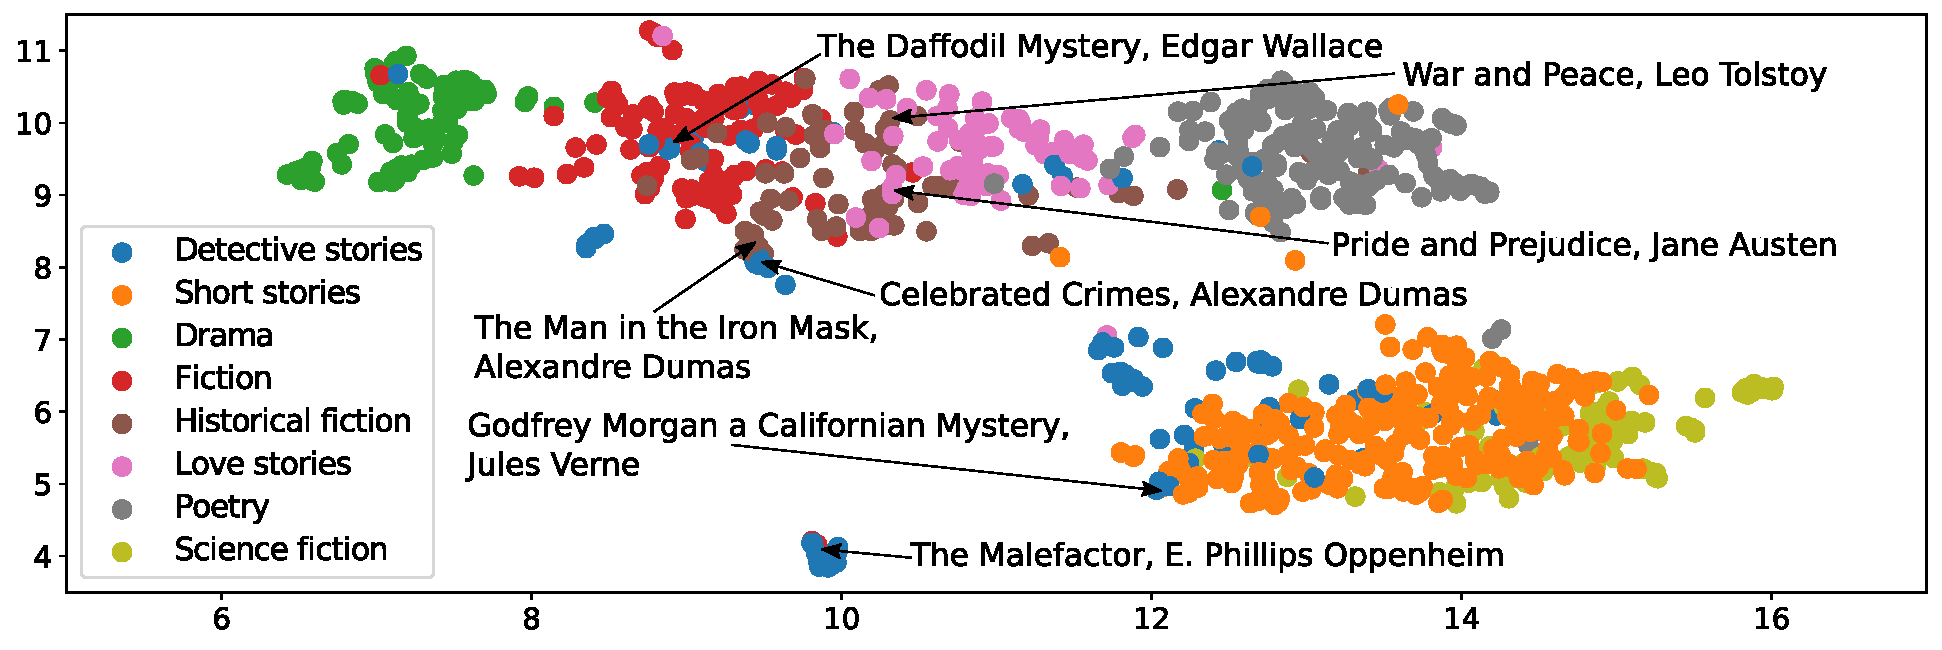
\includegraphics[width=\textwidth]{figures/plot_genres_multi_column.pdf}
	\caption{UMAP projection of the facet \textit{plot} of \emph{lib2vec} trained on the MGG corpus.}
	\label{fig:plot_genres_multi_column}
\end{figure*}

We also performed an extensive qualitative evaluation of the \emph{lib2vec} model with respect to aggregated representation and individual facet embeddings in collaboration with domain experts from literary sciences.
Figure~\ref{fig:plot_genres_multi_column} depicts a UMAP visualization of the embedding space of the plot facet for the MGG corpus. The different colors indicate the genre of the novels.
Note that the plots of the detective stories is scattered across multiple genre clusters and that,e.g., historical fiction has some overlap with love stories.


\section{Conclusions \& Future Work}

Traditional embedding algorithms have an input sequence limit for the efficient encoding of documents.
Long texts, such as novels, often exceed these limits.
Therefore, not all available information is used when embedding long documents, or the long documents are split sequencially into smaller chunks.
Both solutions result in sub-optimal performance on a variety of tasks regarding long documents.
We introduced \emph{lib2vec}, a multi-faceted document embedding framework that splits long documents not sequencially but semantically based on domain-specific facets.
It provides semantically more meaningful document representations than truncation- or chunk-based methods.
%We were able to show the effectiveness of our approach in several experiments.
%Due to the lack of benchmark datasets, we conducted a survey on book similarities to create the BoCo dataset.
%Aside from that, we also used meta-data, such as series associations, author names, and genre labels.
Our approach outperforms baselines, such as doc2vec, BERT, or P-SIF for corpora that contain large- and medium-sized novels on classification tasks, rating prediction, and assessing similarities.
%However, \emph{lib2vec} was not able to exceed the performance of traditional and state-of-the-art embeddings on shorter documents.
%We have also shown that our model outperforms others in classification tasks, such as predicting high-rated books.

The most interesting question for future work is how to incorporate additional knowledge into our model, e.g., by pre-training and/or fine-tuning.
Large language models encode semantic knowledge that we aim to utilize for facet computation in the future.
We further want to test \emph{lib2vec} in other domains with other facets, e.g., for long scientific texts, or legal documents.
Also, in the literary domain, there are facets we didn't explore yet, such as readability~\cite{feng_2010} or literariness~\cite{van_2019}.



%%
%% The acknowledgments section is defined using the "acks" environment
%% (and NOT an unnumbered section). This ensures the proper
%% identification of the section in the article metadata, and the
%% consistent spelling of the heading.
%\begin{acks}
%To Robert, for the bagels and explaining CMYK and color spaces.
%\end{acks}

%%
%% The next two lines define the bibliography style to be used, and
%% the bibliography file.
\bibliographystyle{ACM-Reference-Format}
\bibliography{bib}

%%
%% If your work has an appendix, this is the place to put it.
%\appendix
%
%\section{Research Methods}
%
%\subsection{Part One}
%
%Lorem ipsum dolor sit amet, consectetur adipiscing elit. Morbi
%malesuada, quam in pulvinar varius, metus nunc fermentum urna, id
%sollicitudin purus odio sit amet enim. Aliquam ullamcorper eu ipsum
%vel mollis. Curabitur quis dictum nisl. Phasellus vel semper risus, et
%lacinia dolor. Integer ultricies commodo sem nec semper.

\end{document}
\endinput
%%
%% End of file `sample-sigconf.tex'.
